%!TEX root = ../thesis.tex

\chapter[appendix for benchmarking generative latent variable models for speech]{Benchmarking Generative Latent Variable Models for Speech}
\label{app:supplementary-benchmarking_workshop}
\ifthenelse{\equal{\skipappendices}{true}}{}{


\section{Reproducibility statement}\label{app: reproducibility statement}
The source code used for the work presented in this paper will be made available before the conference. 
This code provides all details, practical and otherwise, needed to reproduce the results in this paper including data preprocessing, model training, model likelihood and latent space evaluation.
The source code also includes scripts for downloading and preparing the LibriSpeech, LibriLight and TIMIT datasets. The LibriSpeech and LibriLight datasets are open source and can be downloaded with the preparation scripts. They are also available at \url{https://www.openslr.org/12} and \url{https://github.com/facebookresearch/libri-light}, respectively. The TIMIT dataset is commercial and must be purchased and downloaded from \url{https://catalog.ldc.upenn.edu/LDC93S1} before running the preparation script.

The stochastic latent variable models considered in this work do not provide an exact likelihood estimate nor an exact latent space representation. For the likelihood, they provide a stochastic lower bound and some variation in the reproduced likelihoods as well as latent representations must be expected between otherwise completely identical forward passes. This variance is fairly small in practice when averaging over large datasets such as those considered in this work. We seed our experiments to reduce the randomness to a minimum, but parts of the algorithms underlying the CUDA framework are stochastic for efficiency. To retain computational feasibility, we  do not run experiments with a deterministic CUDA backend.


\section{Ethics statement}\label{app: ethics statement}
The work presented here fundamentally deals with automated perception of speech and generation of speech. These applications of machine learning potentially raise a number of ethical concerns. For instance, the these models might see possibly adverse use in automated surveillance and generation of deep fakes. To counter some of these effects, this work has focused on openness by using publicly available datasets for model development and benchmarking. Additionally, the work will open source the source code used to create these results. 
Ensuring the net positive effect of the development of these technologies is and must continue to be an ongoing effort.

We do not associate any significant ethical concerns with the datasets used in this work. However, one might note that the TIMIT dataset has somewhat skewed distributions in terms of gender and race diversity. Specifically, the male to female ratio is about two to one while the vast majority of speakers are Caucasian. Such statistics might have an effect of some ethical concern on downstream applications derived from such a dataset as also highlighted in recent research \parencite{koenecke_racial_2020}. In LibriSpeech, there is an approximately equal number of female and male speakers while the diversity in race is unknown to the authors.


\section{Datasets}\label{app: dataset details}
\paragraph{TIMIT} 
TIMIT \parencite{garofolo_timit_1993} is a speech dataset which contains $\SI{16}{kHz}$ recordings of 630 speakers of eight major dialects of American English, each reading ten phonetically rich sentences. It amounts to 6300 total recordings splits approximately in 3.94 hours of audio for training and 1.43 hours of audio for testing. No speakers or sentences in the test set are in the training set. 
The full train and test subsets of TIMIT are as in previous work \parencite{chung_recurrent_2015, fraccaro_sequential_2016, aksan_stcn_2019}. 
We randomly sample 5\% of the training set to use as a validation set. 
TIMIT includes temporally aligned annotations of phonemes and words as well as speaker metadata such as gender, height, age, race, education level and dialect region \parencite{garofolo_timit_1993}.

\paragraph{LibriSpeech and LibriLight}
The LibriSpeech dataset \parencite{panayotov_librispeech_2015} consists of readings of public domain audio books amounting to approximately $\SI{1000}{h}$ of audio. The data is derived from the LibriVox project.
LibriLight \parencite{kahn_libri-light_2020} is a subset of LibriSpeech created as an automatic speech transcription (ASR) benchmark with limited or no supervision.
We specifically train on the $\SI{100}{h}$ \textrm{train-clean-100} subset of LibriSpeech and the $\SI{10}{h}$ subset of LibriLight. 
In all cases we evaluate on all the test splits \textrm{dev-clean}, \textrm{dev-other}, \textrm{test-clean}, \textrm{test-other}.

Both datasets represent the audio as $\SI{16}{bit}$ pulse code modulation (PCM) sampled at $\SI{16000}{Hz}$.


\section{Model architectures}\label{app: model architectures}
This section details model architectures. See appendix~\cref{app: additional graphical models} for graphical models and appendix~\cref{app: training details} for training details. 

\paragraph{WaveNet}
We implement WaveNet as described in the original work \parencite{oord_wavenet_2016} but use a discretized mixture of logistics as the output distribution as also done in other work \parencite{oord_parallel_2018}. Our WaveNet is not conditioned on any signal other than the raw waveform. The model applies the causal convolution directly to the raw waveform frames (i.e. one input channel). An alternative option that we did not examine is to replace the initial convolution with an embedding lookup with a learnable vector for each waveform frame value.

\paragraph{LSTM}
The LSTM baseline uses an MLP encoder to embed the waveform subsegment $\vx_{t:t+s-1}$ to a feature vector before feeding it to the LSTM cell. The encoder is similar to the parameterization of $\phi_\text{vrnn}^\text{enc}$ for the VRNN described above. The LSTM cell produces the hidden state $\vd_t$ from $\vx_{t:t+s-1}$ and passes it to a decoder. Like the encoder, the decoder is parameterized like $\phi_\text{vrnn}^\text{dec}$ of the VRNN. It outputs the waveform predictions $\vx_{t+s:t+2s-1}$ from the hidden state $\vd_t$. The LSTM model uses a single vanilla unidirectional LSTM cell. 

\paragraph{VRNN}
We implement the VRNN as described in the original work \parencite{chung_recurrent_2015} and verify that we can reproduce the original Gaussian likelihood TIMIT results. We replace the Gaussian output distribution with the DMoL. 

\paragraph{SRNN}
We implement the VRNN as described in the original work \parencite{fraccaro_sequential_2016} and verify that we can reproduce the original Gaussian likelihood TIMIT results. We replace the Gaussian output distribution with the DMoL. 

\paragraph{CW-VAE} We implement the CW-VAE based on the original work \parencite{saxena_clockwork_2021} but with some modifications also briefly described in the paper. We replace the encoder/decoder model architectures of the original work with architectures designed for waveform modeling. Specifically, the encoder and decoder are based on the Conv-TasNet \parencite{luo_conv-tasnet_2019} and uses similar residual block structure. However, contrary to the Conv-TasNet, we require downsampling factors larger than two. In order to achieve this we use strides of two in the separable convolution of each block. With e.g. six blocks we hence get an overall stride of $2^6=64$. We can then add additional blocks with unit stride.
We also need to modify the residual connections that skip strided convolutions. Specifically, we replace the residual with a single convolution with stride equal to the stride used in the separable convolution. This convolution uses no nonlinearity and hence simply learns a local linear downsampling.

\paragraph{STCN} We implement the STCN as described in the original work \parencite{aksan_stcn_2019} and verify that we can reproduce the original Gaussian likelihood TIMIT results. We replace the Gaussian output distribution with the DMoL. We use the best-performing version of the STCN reported in the original paper, namedly the ``STCN-dense" variant which conditions the observed variable on all five latent variables in the hierarchy. For the ablation experiment, we remove the bottom four latent variables. That is, we completely remove the corresponding four small densely connected networks that parameterize the prior and posterior distributions based on deterministic representations of the WaveNet encoder. We keep the top most prior and posterior networks and use them to parameterize a latent variable of $256$. This maintains the widest bottleneck of the model as well as almost all of the model's capacity.

\paragraph{ASR model}
The ASR model used for the phoneme recognition experiments is a three-layered bidirectional LSTM. We apply temporal dropout between the LSTM layers and also after the final layer. Temporal dropout works similar to regular dropout but samples the entries of the hidden state to mask only once and apply it to all timesteps, i.e. masking $\vh_{t}$ at vector index $i$ for all $t$ (and $i$). 
We mask by zeroing vector elements. We never mask the first timestep. 
We apply temporal dropout with masking probability of 0.3 for the 3.7h subset, 0.35 for the 1h subset and 0.4 for the 10m subset. 
The only difference in model architecture between the evaluation of different representations is the first affine transformation; from the dimensionality of the representation to the hidden state size of the LSTM. This gives rise to a very small difference in model capacity and parameter count which we find is negligible. We set the hidden unit size to 256. 


\section{Training details}\label{app: training details}
\paragraph{Likelihood benchmark}
We implement all models and training scripts in PyTorch 1.9 \parencite{paszke_automatic_2017}.
For both datasets we use the Adam optimizer \parencite{kingma_adam_2015} with default parameters as given in PyTorch. We use learning rate $3\text{e}-4$ and no learning rate schedule.
We use PyTorch automatic mixed precision (AMP) to significantly reduce memory consumption. We did not observe any significant difference in final model performance compared to full ($\SI{32}{bit}$) precision.

We train stateful models (LSTM, VRNN, SRNN and CW-VAE) on the full sequence lengths padding batches with zeros when examples are not of equal length. We sample batches such that they consist of examples that are approximately the same length to minimize the amount of computation wasted on padding.

For $s=1$, we train stateless models (WaveNet, STCN) on random subsegments of the training examples and resample every epoch. This reduces memory requirements but does not bias the gradient. The subsequences are chosen to be of length 16000 which is larger than the receptive fields of the models and corresponds to one second of audio in TIMIT and LibriSpeech. 
For $s=64$ and $s=256$ we train the stateless models on the full example lengths similar to the stateful models since the receptive field is effectively $s$ times larger and the shorter sequence length reduces memory requirements.

In testing, we evaluate on the full sequences. Due to memory constrains, for LibriSpeech, we need to split the test examples into subsegments since the average sequence length in Librispeech is about 4 times longer than that of TIMIT. Hence, we do multiple forward passes per test example, one for each of several subsegments. We carry along the internal state for models that are autoregressive in training (LSTM, VRNN, SRNN, CW-VAE) and define segments to overlap according to model architecture.

\paragraph{Phoneme recognition}
The ASR experiment consists of two stages: 1) pre"=training of the unsupervised model and 2) training of the ASR model. The pre"=training is done as for the likelihood benchmark above. The ASR model is trained using the Adam optimizer \parencite{kingma_adam_2015} with default parameters as given in PyTorch. We use learning rate $3\text{e}-4$ and no learning rate schedule. 

For the spectrogram, WaveNet and the LSTM, we extract the representation only once and train the ASR model on these. Since the models are deterministic and do not parameterize distributions, this is the only option. For the LVMs, we resample the latent representation of a training example at every epoch. This is the most principled approach as these models parameterize probability distributions. Furthermore, using a single sample would be subject to artificially high variance in the representations while it is not straightforward to establish a sound mean representation for sequential models.




\section{Converting the likelihood to units of bits per frame}\label{app: likelihood in bits per frame}
Here we briefly describe how to compute a likelihood in units of bits per frame (bpf). In the main text, we use $\log$ to mean $\log_e$, but here we will be explicit. In general, conversion from nats to bits (i.e., from $\log_e$ to $\log_2$) is achieved by $\log_2(x) = \log_e(x)  / \log_2(e) $. Remember that $\log_2 p(\vx_{1:T})$ generally factorizes as $\sum_t \log_2 p(x_t|\cdot)$. In sequence modeling, it is important to remember that each example $\vx^{i}$ must be weighted differently according the sequence length of that specific example. This is in contrast to computing bits per dimension in the image domain where images in a dataset are usually of the same dimensions. Thus, we compute the log-likelihood in bits per frame over the entire dataset as
\begin{equation}
    \mathcal{L}(\vx^{i}) = \frac{1}{\sum_i T_i} \sum_i \sum_t \log_2 p(\vx_t^{i}) \enspace ,
\end{equation}
where $i$ denotes the example index, $T_i$ is the length of example $\vx^i$ in waveform frames and $t$ is the time index. If a single timestep $\vx_t^i$ represents multiple waveform frames stacked with some stack size $s$, it is important to note that the sum over $t$ only has $T_i/s$ elements. 
For the LVMs, the term $\log_2 p(\vx_t^{i})$ is lower bounded by the ELBO in \eqref{eq: elbo}. 


\section{Additional likelihood results} \label{app: additional likelihood results appendix}

\paragraph{LibriSpeech, $\mu$-law, DMoL} We provide additional results on LibriSpeech with audio represented as $\mu$-law encoded PCM in \cref{tab: likelihoods librispeech}. See appendix~\cref{app: dataset details}, \cref{app: model architectures} and \cref{app: training details} for additional details.

\paragraph{TIMIT, $\mu$-law, DMoL} We provide additional results on TIMIT with audio represented as $\mu$-law encoded PCM in \cref{tab: timit likelihoods dmol mu-law appendix}. Details are as presented in the main paper.

\paragraph{TIMIT, linear, DMoL}: We provide results on TIMIT with audio represented as linear PCM (raw PCM) in \cref{tab: timit likelihoods dmol linear appendix}. Except for the encoding, details are as for $\mu$-law encoded TIMIT

\paragraph{TIMIT, linear, Gaussian} We also provide some results on TIMIT with the audio instead represented as linear PCM (linearly encoded) and using Gaussian output distributions as has been done previously in the literature \parencite{chung_recurrent_2015, fraccaro_sequential_2016, lai_stochastic_2018, aksan_stcn_2019}. We use $s=200$ for comparability to the previous work. We provide the results in \cref{tab: timit likelihoods gaussian appendix} and include likelihoods reported in the literature for reference. For our models, we use the same architectures as before but replace the discretized mixture of logistics with either a Gaussian distribution or a mixture of Gaussian distributions. 

We constrain the standard deviation of the Gaussians used with our models to be at least $\sigma_\text{min} = 0.01$ in order to avoid it going to zero, the likelihood going to infinity and optimization becoming unstable. The minimum Gaussian standard deviation of \textcite{aksan_stcn_2019} is $\sigma_\text{min} = 0.001$.

From \cref{tab: timit likelihoods gaussian appendix} we note that the performance of the CW-VAE with Gaussian output distribution when modeling linear PCM (i.e. not $\mu$-law encoded) does not compare as favorably to the other baselines as it did with the discretized mixture of logistics distribution. We hypothesize that this has to do with using a Gaussian output distribution in latent variable models which, as has been reported elsewhere \parencite{mattei_leveraging_2018}, leads to a likelihood function that is unbounded above and can grow arbitrarily high. We discuss this phenomenon in further detail in section~\cref{app: gaussian likelihood unboundedness discussion}. 

We specifically hypothesize that models that are autoregressive in the observed variable (VRNN, SRNN, Stochastic WaveNet, STCN) are well-equipped to utilize local smoothness to put very high density on the correct next value and that this in turn leads to a high degree of exploitation of the unboundedness of the likelihood. Not being autoregressive in the observed variable, the CW-VAE cannot exploit this local smoothness in the same way. Instead, the reconstruction is conditioned on a stochastic latent variable, $p(\vx_t|\vz^1_t)$, which introduces uncertainty and likely larger reconstruction variances.


\begin{table*}[t]
    \caption{
    Model likelihoods $\mathcal{L}$ on \textbf{LibriSpeech} test sets represented as \textbf{16 bit $\boldsymbol{\mu}$-law encoded PCM}.
    For the CW-VAE, $s$ refers to $s_1$ and the two-layered models have $s_2=8s_1$.
    The models are trained on either the $\SI{10}{h}$ LibriLight subset or the $\SI{100}{h}$ LibriSpeech \textrm{train-clean-100} subset as indicated.
    Likelihoods are given in units of bits per frame (bpf).
    }
    \centering
    \resizebox{0.98\textwidth}{!}{
    \begin{tabular}{lll|rrrr}  % https://wandb.ai/vseq/icml_asr
        \toprule
        $s$ & \bf Model                   & \bf Configuration       & \multicolumn{4}{c}{\bf Likelihood $\mathcal{L}$ [bpf]} \\
         & & & dev-clean & dev-other & test-clean & test-other\\
         & & & 10h/100h & 10h/100h & 10h/100h & 10h/100h\\
        \midrule
        1 & Uniform             & Uninformed     & \multicolumn{1}{c}{16.00} & \multicolumn{1}{c}{16.00} & \multicolumn{1}{c}{16.00} & \multicolumn{1}{c}{16.00} \\
        1 & DMoL                & Optimal        & \multicolumn{1}{c}{15.66} & \multicolumn{1}{c}{15.70} & \multicolumn{1}{c}{15.62} & \multicolumn{1}{c}{15.71}\\   % $\vmu=[-0.551, 0.551], \vz=[0.11, 0.11]$
        - & FLAC                & Linear PCM     & \multicolumn{1}{c}{\bf 9.390} & \multicolumn{1}{c}{\bf 9.292} & \multicolumn{1}{c}{\bf 9.700} & \multicolumn{1}{c}{\bf 9.272} \\
        \midrule
        1 & Wavenet             & $D_c=96$       & \bf 10.96/10.89 & \bf 10.85/10.76 & \bf 11.12/11.01 & \bf 11.05/10.85 \\
        1 & LSTM                & $D_d=256$      & 11.21/11.17 & 11.10/11.06 & 11.35/11.29 & 11.28/11.23 \\  % 15ua3hau/(lmssrk5k,248n2ylu)
        \midrule
        64 & Wavenet            & $D_c=96$       & 13.61/13.24 & 13.58/13.21 & 13.61/13.22 & 13.60/13.21 \\  % 2ghkybtd/3iieasdt
        64 & LSTM               & $D_d=256$      & 13.56/13.25 & 13.52/13.24 & 13.55/13.23 & 13.56/13.25 \\  % 10fpovu3/2bu1izin
        64 & CW-VAE             & $D_z=96,L=1$   & $\leq$12.32/12.24 & 12.32/12.23 & 12.43/12.33 & 12.43/12.33 \\
        64 & CW-VAE             & $D_z=96,L=2$   & $\leq$12.30/12.22 & 12.30/12.21 & 12.40/12.31 & 12.39/12.32 \\
        64 & STCN               & $D_z=256,L=5$  & $\leq$\bf 11.83/11.47 & \bf 11.82/11.46 & \bf 11.94/11.58 & \bf 11.94/11.60 \\  % kutxm2hx/3t0xg7pb
        \bottomrule
    \end{tabular}
    }
    \label{tab: likelihoods librispeech}
\end{table*}


\begin{table}[t!]
    \caption{
    Model likelihoods on TIMIT represented as a 16 bit linear PCM, obtained by different latent variable models and compared to autoregressive baselines all using a discretized mixture of logistics with 10 components as output distribution. Likelihoods are given in units of bits per frame (bpf) and obtained by normalizing the total likelihood of each sequence with the individual sequence length and then averaging over the dataset. The STCN converges to a poor local minimum and sometimes diverges when modeling linear PCM with $s=1$.
    }
    \centering
    \begin{tabular}{lll|r}
        \toprule
        $s$    & \bf Model              & \bf Configuration     & \bf $\mathcal{L}$ [bpf] \\
        \midrule
        1         & Uniform             & Uninformed            & 16.00 \\
        1         & DMoL                & Optimal               & 10.70 \\   % $mean[0.00], scale=[0.005]$
        %-         & FLAC                & Linear PCM            & 8.582 \\
        \midrule
        $1$       & Wavenet             & $D_C=96$              & \textbf{7.246} \\
        $1$       & LSTM                & $D_d=256, L=1$        & 7.295 \\
        $1$       & VRNN                & $D_z=256$             & $\leq$7.316 \\
        $1$       & SRNN                & $D_z=256$             & $\leq$7.501 \\
        $1$       & STCN                & $D_z=256,L=5$         & $\leq$9.970 \\
        \midrule
        $64$      & WaveNet             & $D_c=96$              & 8.402 \\
        $64$      & LSTM                & $D_d=256, L=1$        & 8.357 \\
        $64$      & VRNN                & $D_z=256$             & $\leq$8.103 \\
        $64$      & SRNN                & $D_z=256$             & $\leq$8.036 \\
        $64$      & CW-VAE              & $D_z=96, L=1$         & $\leq$7.989 \\
        % $64$      & CW-VAE              & $D_z=96, L=2$         & $\leq$XX \\
        % $64$      & CW-VAE              & $D_z=96, L=3$         & $\leq$XX \\
        $64$      & STCN                & $D_z=256,L=5$  & $\leq$\textbf{7.768} \\
        \midrule
        $256$      & WaveNet             & $D_c=96$              & 9.018 \\
        $256$      & LSTM                & $D_d=256, L=1$        & 8.959 \\  % overfits slightly
        $256$      & VRNN                & $D_z=256$             & $\leq$8.739 \\
        $256$      & SRNN                & $D_z=256$             & $\leq$8.674 \\
        $256$      & CW-VAE              & $D_z=96, L=1$         & $\leq$8.406 \\
        % $256$      & CW-VAE              & $D_z=96, L=2$         & $\leq$XX \\
        % $256$      & CW-VAE              & $D_z=96, L=3$         & $\leq$XX \\
        $256$      & STCN                & $D_z=256,L=5$         & $\leq$\textbf{8.196} \\
        \bottomrule
    \end{tabular}
    \label{tab: timit likelihoods dmol linear appendix}
\end{table}


\begin{table}[p]
    \caption{
    Model likelihoods on TIMIT represented as a \textbf{16 bit $\boldsymbol{\mu}$-law encoded PCM}, obtained by different latent variable models and compared to autoregressive baselines all using a discretized mixture of logistics with 10 components as output distribution. Likelihoods are given in units of bits per frame (bpf) and obtained by normalizing the total likelihood of each sequence with the individual sequence length and then averaging over the dataset.
    }
    \centering
    \begin{tabular}{lll|r}
        \toprule
        $s$    & \bf Model           & \bf Configuration           & \bf $\mathcal{L}$ [bpf] \\
        \midrule
        $1$       & Wavenet             & $D_C=16$              & 11.27 \\
        $1$       & Wavenet             & $D_C=24$              & 11.14 \\
        $1$       & Wavenet             & $D_C=32$              & 11.03 \\
        $1$       & Wavenet             & $D_C=96$              & 10.88 \\
        $1$       & Wavenet             & $D_C=128$             & 10.98 \\
        $1$       & Wavenet             & $D_C=160$             & 10.91 \\
        $1$       & LSTM                & $D_d=128, L=1$        & 11.40 \\
        $1$       & LSTM                & $D_d=256, L=1$        & 11.11 \\
        $1$       & VRNN                & $D_z=256$             & $\leq$11.09 \\
        $1$       & SRNN                & $D_z=256$             & $\leq$11.19 \\
        1 & STCN                & $D_z=256,L=5$               & $\leq$11.77 \\  % 39u25hyi
        \midrule
        $4$       & LSTM                & $D_d=256, L=1$        & 11.65 \\
        \midrule
        $16$      & LSTM                & $D_d=256, L=1$        & 12.54 \\
        $16$      & LSTM                & $D_d=256, L=2$        & 12.54 \\
        $16$      & LSTM                & $D_d=256, L=3$        & 12.44 \\
        \midrule
        $64$      & WaveNet             & $D_c=96$              & 13.30 \\
        $64$      & LSTM                & $D_d=96, L=1$         & 13.49 \\
        $64$      & LSTM                & $D_d=96, L=2$         & 13.46 \\
        $64$      & LSTM                & $D_d=96, L=3$         & 13.40 \\
        $64$      & LSTM                & $D_d=256, L=1$        & 13.27 \\
        $64$      & LSTM                & $D_d=256, L=2$        & 13.29 \\
        $64$      & LSTM                & $D_d=256, L=3$        & 13.31 \\
        $64$      & LSTM                & $D_d=512, L=1$        & 13.37 \\
        $64$      & LSTM                & $D_d=512, L=2$        & 13.37 \\
        $64$      & LSTM                & $D_d=512, L=3$        & 13.41 \\
        $64$      & VRNN                & $D_z=96$              & $\leq$12.93 \\
        $64$      & VRNN                & $D_z=256$             & $\leq$12.54 \\
        $64$      & SRNN                & $D_z=96$              & $\leq$12.87 \\
        $64$      & SRNN                & $D_z=256$             & $\leq$12.42 \\
        $64$      & CW-VAE              & $D_z=96, L=1$         & $\leq$12.44 \\
        $64$      & CW-VAE              & $D_z=96, L=2$         & $\leq$12.17 \\
        $64$      & CW-VAE              & $D_z=96, L=3$         & $\leq$12.15 \\
        $64$      & CW-VAE              & $D_z=256, L=2$        & $\leq$12.10 \\
        $64$ & STCN               & $D_z=256,L=1$               & $\leq$12.32 \\  % 2ss9fvxd
        $64$ & STCN               & $D_z=256,L=5$               & $\leq$11.78 \\
        \midrule
        $256$     & WaveNet             & $D_c=96$              & 14.11 \\
        $256$     & LSTM                & $D_d=256, L=1$        & 14.20 \\
        $256$     & LSTM                & $D_d=256, L=2$        & 14.17 \\
        $256$     & LSTM                & $D_d=256, L=3$        & 14.26 \\
        $256$     & VRNN                & $D_z=96$              & $\leq$13.51 \\
        $256$     & VRNN                & $D_z=256$             & $\leq$13.27 \\
        $256$     & SRNN                & $D_z=96$              & $\leq$13.28 \\
        $256$     & SRNN                & $D_z=256$             & $\leq$13.14 \\
        $256$     & CW-VAE              & $D_z=96, L=1$         & $\leq$13.11 \\
        $256$     & CW-VAE              & $D_z=96, L=2$         & $\leq$12.97 \\
        $256$     & CW-VAE              & $D_z=96, L=3$         & $\leq$12.87 \\
        $256$ & STCN              & $D_z=256,L=1$               & $\leq$13.07 \\  % 2h5ns3zw
        $256$ & STCN              & $D_z=256,L=5$               & $\leq$12.52 \\
        \bottomrule
    \end{tabular}
    \label{tab: timit likelihoods dmol mu-law appendix}
\end{table}


\begin{table}[t!]
    \caption{
    Model likelihoods on TIMIT represented as globally normalized 16 bit linear PCM. Likelihoods are given in units of nats and obtained by summing the likelihood over time and over all examples in the dataset and dividing by the total number of examples. In the table, Normal refers to using a Gaussian likelihood and GMM refers to using a  Gaussian Mixture Model likelihood with 20 components. Models with asterisks $^*$ are our implementations while remaining results are as reported in the referenced work.
    }
    \centering
    \begin{tabular}{lll|r}
        \toprule
        $s$ & \bf Model           & \bf Configuration           & \bf $\mathcal{L}$ [nats] \\
        \midrule
        1 & WaveNet                                                               & Normal & 119656 \\
        1 & WaveNet                                                               & GMM-2  & 120699 \\
        1 & WaveNet                                                               & GMM-20 & 121681 \\
        \midrule
        % 200 & WaveNet                                                              & GMM    & XX.XX
        200 & WaveNet {\scriptsize \parencite{aksan_stcn_2019}}                        & GMM-20    & 30188 \\
        200 & WaveNet {\scriptsize \parencite{aksan_stcn_2019}}                        & Normal & -7443 \\
        200 & Stochastic WaveNet$^*$ {\scriptsize \parencite{lai_stochastic_2018}}     & Normal & $\geq$72463\\
        % 200 & VRNN {\scriptsize \parencite{chung_recurrent_2015}}                          & & \\
        200 & VRNN {\scriptsize \parencite{chung_recurrent_2015}}                      & Normal & $\approx$28982\\
        % 200 & SRNN {\scriptsize \parencite{fraccaro_sequential_2016}}                      & & \\
        200 & SRNN {\scriptsize \parencite{fraccaro_sequential_2016}}                  & Normal & $\geq$60550 \\
        200 & STCN {\scriptsize \parencite{aksan_stcn_2019}}                           & GMM-20 & $\geq$69195\\
        200 & STCN {\scriptsize \parencite{aksan_stcn_2019}}                           & Normal & $\geq$64913\\
        200 & STCN-dense {\scriptsize \parencite{aksan_stcn_2019}}                     & GMM-20 & $\geq$71386\\
        200 & STCN-dense {\scriptsize \parencite{aksan_stcn_2019}}                     & Normal & $\geq$70294\\
        200 & STCN-dense-large {\scriptsize \parencite{aksan_stcn_2019}}               & GMM-20 & $\geq$77438\\
        200 & CW-VAE$^*$                                         & $L=1, D_z=96$, Normal & $\geq$41629 \\  % https://wandb.ai/vseq/cwvae/runs/n8nu778t?workspace=user-jaksen
        % 200 & CW-VAE$^*$                                         & $L=2, D_z=96$, Normal & $\geq$2090 \\  % https://wandb.ai/vseq/cwvae/runs/1so36fii?workspace=user-jaksen
        \bottomrule
    \end{tabular}
    \label{tab: timit likelihoods gaussian appendix}
\end{table}


\section{Additional discussion on Gaussian likelihoods in LVMs} \label{app: gaussian likelihood unboundedness discussion}
As noted in section~\cref{app: additional likelihood results appendix}, we constrain the variance of the output distribution of our models to be $\sigma^2_\text{min} = 0.01^2$ for the additional results on TIMIT with Gaussian outputs. This limits the maximum value attainable by the prediction/reconstruction density of a single waveform frame $x_t$. 

Specifically, we can see that since
\begin{equation}
    \log p(x_t|\cdot) = \log \mathcal{N}\pa{x_t; \mu_t, \max\cbra{\sigma_\text{min}^2, \sigma_t^2}}\enspace \label{eq: gaussian ll with minimum variance} ,
\end{equation}
the best prediction/reconstruction density is achieved when $\sigma^2 \leq \sigma_\text{min}^2$ and $\mu=x_t$. 
Here $\cdot$ indicates any variables we might condition on such as the previous input frame $x_{t-1}$ or some latent variables.
We can evaluate this best case scenario for $\sigma_\text{min}^2 = 0.01^2$,
\begin{align}
    \log \mathcal{N}\pa{x_t; x_t, \sigma_\text{min}^2} &= -\frac{1}{2}\log 2\pi - \frac{1}{2}\log \sigma_\text{min}^2 - \frac{1}{2\sigma_\text{min}^2} (x_t - x_t) \nonumber \\
    &= -\frac{1}{2}\log 2\pi - \frac{1}{2}\log 0.01^2 \nonumber \\
    &= 3.686 \enspace . 
\end{align}
Hence, with perfect prediction/reconstruction and the minimal variance ($0.01^2$), a waveform frame contributes to the likelihood with $\SI{3.686}{nats}$. With an average test set example length of $\SI{49367.3}{frames}$ frames this leads to a best-case likelihood of 181967. We provide a list of maximally attainable Gaussian likelihoods on TIMIT for different minimal variances in \cref{tab:timit best gaussian ll}. One can note that the maximal likelihood at $\sigma_\text{min}^2=0.1^2$ is lower than the likelihoods achieved by some models in \cref{tab: timit likelihoods gaussian appendix}. This indicates that the models learn to use very small variances in order to increase the likelihood. Empirically, standard deviations smaller than approximately $0.001$ can result in numerical instability.


\begin{table}[t!]
    \caption{The highest possible Gaussian log-likelihoods (max $\mathcal{L}$) attainable on the TIMIT test set as computed by \eqref{eq: gaussian ll with minimum variance} with different values of the minimum variance $\sigma^2_\text{min}$.}
    \centering
    \begin{tabular}{rrr}
    \toprule
    $\sigma_\text{min}$ & $\sigma_\text{min}^2$ & $\max\mathcal{L}$ \\
    \midrule
    $1$      & $1$           &    $-45367$ \\
    $0.5$    & $0.25$        &    $-11146$ \\
    $0.1$    & $0.01$        &     $68307$ \\
    $0.05$   & $0.0025$      &    $102525$ \\
    $0.01$   & $0.0001$      &    $181979$ \\
    $0.005$  & $0.000025$    &    $216198$ \\
    $0.001$  & $0.000001$    &    $295651$ \\
    \bottomrule
    \end{tabular}
    \label{tab:timit best gaussian ll}
\end{table}




\section{Additional discussion on the choice of output distribution}\label{app: additional discussion on output distribution}
The DMoL uses a discretization of the continuous logistic distribution to define a mixture model over a discrete random variable. This allows it to parameterize multimodal distributions which can express ambiguity about the value of $\vx_t$.
The model can learn to maximize likelihood by assigning a bit of probability mass to multiple potential values of $\vx_t$.

While this is well-suited for autoregressive modeling, for which the distribution was developed, the potential multimodality poses a challenge for non"=autoregressive latent variable models which independently sample multiple neighboring observations at the output.
In fact, if multiple neighboring outputs defined by the subsequence $\vx_{t_1:t_2}$ have multimodal $p(\vx_t|\cdot)$, we risk sampling a subsequence where each neighboring value expresses different potential realities, independently. 

Interestingly, most work on latent variable models with non"=autoregressive output distributions seem to ignore this fact and simply employ the mixture distribution with 10 mixture components \parencite{maaloe_biva_2019, vahdat_nvae_2020, child_very_2021}.
However, given the empirically good results of latent variable models for image generation, this seems to have posed only a minor problem in practice. We speculate that this is due to the high degree of similarity between neighbouring pixels in images. I.e. if the neighboring pixels are nuances of red, then, in all likelihood, so is the central pixel.

In the audio domain, however, neighbouring waveform frames can take wildly different values, especially at low sample rates. Furthermore, waveforms exhibit a natural symmetry between positive and negative amplitudes.
Hence, it seems plausible that multimodality may pose a larger problem in non"=autoregressive speech generation by causing locally incoherent samples than it seems to do in image modelling.


\section{Additional graphical models}\label{app: additional graphical models}
In \cref{fig: cwvae cell state graph} we show the graphical model of the recurrent cell of the CW-VAE for a single time step. As noted in \parencite{saxena_clockwork_2021}, this cell is very similar to the one of the Recurrent State Space Model (RSSM) \parencite{hafner_learning_2019}.

In \cref{fig: cwvae three-layered graphical models (inference and generative)} we show the unrolled graphical models of a three-layered CW-VAE with $k_1=1$ and $c=2$ yielding $k_2=2$ and $k_3=4$. 
We show both the generative and inference models and highlight in blue the parameter sharing between the two models due to top-down inference.

In \cref{fig: stcn graphical models (inference and generative)} we show the graphical models of the STCN \parencite{aksan_stcn_2019} at a single timestep. The model has three layers and shares the parameters of the WaveNet encoder between the inference and generative models.

In \cref{fig: vrnn graphical models (inference and generative)} we illustrate the unrolled graphical models of the inference and generative models of the VRNN \parencite{chung_recurrent_2015}. We include the deterministic variable $\vd_t$ in order to illustrate the difference to other latent variable models.

Likewise, in \cref{fig: srnn graphical models (inference and generative)} we illustrate the unrolled graphical models the SRNN \parencite{fraccaro_sequential_2016}.


\begin{figure}[t!]
    \centering
    \def\col{blue}
    \begin{tikzpicture}
        % LATENT STATE SEGMENTATION
        % internal latent state
        \node[det] (h_t_l) {$\vd_t^l$};
        \node[latent, below right=1cm of h_t_l] (z_t_l) {$\vz_t^l$};
        \node[latent, right=1.5cm of h_t_l] (s_t_l) {$\vs_t^l$};

        % \plate [options] {name} {fitlist} {caption}
        \plate [inner sep=0.4cm] {cell} {(h_t_l)(z_t_l)(s_t_l)} {};
        
        % inputs
        \node[latent,left=0.75cm of h_t_l] (s_tm1_l) {$\vs_{t-1}^l$};
        \node[latent,above=0.75cm of h_t_l] (s_t_lp1) {$\vs_t^{l+1}$};%
        \node[latent,below=1cm of z_t_l] (e_t_l) {$\ve_t^l$};%
        % \node[left=0.5cm of e_t_l] (e_t_l_caption) {($\ve_t^l$ conditioned only in inference)};%
        
        % outputs
        \node[right=1.0cm of s_t_l] (s_t_l_copy1) {};%
        \node[below=2.5cm of s_t_l] (s_t_l_copy2) {};%
        
        % edges
        \edge[blue] {s_tm1_l} {h_t_l}
        \edge[blue] {s_t_lp1} {h_t_l}
        
        \edge[] {h_t_l} {z_t_l}
        \edge[dashed] {e_t_l} {z_t_l}
        
        \edge[blue] {h_t_l} {s_t_l}
        \edge[blue] {z_t_l} {s_t_l}
        
        \edge[blue] {s_t_l} {s_t_l_copy1}
        \edge[blue] {s_t_l} {s_t_l_copy2}
    \end{tikzpicture}
\caption{CW-VAE cell state $\vs_t^l$ update. The cell state is given as $\vs_t^l=(\vz_t^l, \vd_t^l)$ where $\vd_t^l$ is the deterministic hidden state of a Gated Recurrent Unit \parencite{cho_properties_2014}. The vector $\ve_t^l$ is computed from $\vx_t$ by the encoder network which outputs $L$ encodings, one for each latent variable, similar to that of a Ladder VAE \parencite{sonderby_ladder_2016}. All blue arrows are shared between generation and inference. The dashed arrow is used only during inference. The solid arrow has unique transformations during inference and generation.}
\label{fig: cwvae cell state graph}
\end{figure}


\begin{figure}[t!]
    \begin{subfigure}[b]{\textwidth}
    \flushright
    \def\col{blue}
    \resizebox{!}{5.25cm}{
    \begin{tikzpicture}
        % GENERATIVE
        % nodes
        \node[obs] (x_1) {$\vx_t$};%
        \node[obs,right=1.00cm of x_1] (x_2) {$\vx_{t+1}$};%
        \node[obs,right=1.00cm of x_2] (x_3) {$\vx_{t+2}$};%
        \node[obs,right=1.00cm of x_3] (x_4) {$\vx_{t+3}$};%
        \node[obs,right=1.00cm of x_4] (x_5) {$\vx_{t+4}$};%
        \node[obs,right=1.00cm of x_5] (x_6) {$\vx_{t+5}$};%
        \node[obs,right=1.00cm of x_6] (x_7) {$\vx_{t+6}$};%
        \node[obs,right=1.00cm of x_7] (x_8) {$\vx_{t+7}$};%
    
        \node[latent,above=1.00cm of x_1](s_1_1){$\vz^{(1)}_{t}$}; %
        \node[latent,above=1.00cm of x_2](s_1_2){$\vz^{(1)}_{t+1}$}; %
        \node[latent,above=1.00cm of x_3](s_1_3){$\vz^{(1)}_{t+2}$}; %
        \node[latent,above=1.00cm of x_4](s_1_4){$\vz^{(1)}_{t+3}$}; %
        \node[latent,above=1.00cm of x_5](s_1_5){$\vz^{(1)}_{t+4}$}; %
        \node[latent,above=1.00cm of x_6](s_1_6){$\vz^{(1)}_{t+5}$}; %
        \node[latent,above=1.00cm of x_7](s_1_7){$\vz^{(1)}_{t+6}$}; %
        \node[latent,above=1.00cm of x_8](s_1_8){$\vz^{(1)}_{t+7}$}; %
    
        \node[latent,above=1.00cm of s_1_1](s_2_1){$\vz^{(2)}_{t}$}; %
        \node[latent,above=1.00cm of s_1_3](s_2_3){$\vz^{(2)}_{t+2}$}; %
        \node[latent,above=1.00cm of s_1_5](s_2_5){$\vz^{(2)}_{t+4}$}; %
        \node[latent,above=1.00cm of s_1_7](s_2_7){$\vz^{(2)}_{t+6}$}; %
    
        \node[latent,above=1.00cm of s_2_1](s_3_1){$\vz^{(3)}_{t}$}; %
        \node[latent,above=1.00cm of s_2_5](s_3_5){$\vz^{(3)}_{t+4}$}; %
    
        % % x to s first layer
        \edge[]{s_1_1}{x_1};
        \edge[]{s_1_2}{x_2};
        \edge[]{s_1_3}{x_3};
        \edge[]{s_1_4}{x_4};
        \edge[]{s_1_5}{x_5};
        \edge[]{s_1_6}{x_6};
        \edge[]{s_1_7}{x_7};
        \edge[]{s_1_8}{x_8};
    
        % % s per layer forward in time
        \edge[blue]{s_1_1}{s_1_2};
        \edge[blue]{s_1_2}{s_1_3};
        \edge[blue]{s_1_3}{s_1_4};
        \edge[blue]{s_1_4}{s_1_5};
        \edge[blue]{s_1_5}{s_1_6};
        \edge[blue]{s_1_6}{s_1_7};
        \edge[blue]{s_1_7}{s_1_8};
        
        \edge[blue]{s_2_1}{s_2_3};
        \edge[blue]{s_2_3}{s_2_5};
        \edge[blue]{s_2_5}{s_2_7};
        
        \edge[blue]{s_3_1}{s_3_5};
        
        % % s across layers on time
        \edge[blue]{s_2_1}{s_1_1};
        \edge[blue]{s_2_3}{s_1_3};
        \edge[blue]{s_2_5}{s_1_5};
        \edge[blue]{s_2_7}{s_1_7};
    
        \edge[blue]{s_3_1}{s_2_1};
        \edge[blue]{s_3_5}{s_2_5};
        
        % % s across layers forward in time
        \edge[blue]{s_2_1}{s_1_2};
        \edge[blue]{s_2_3}{s_1_4};
        \edge[blue]{s_2_5}{s_1_6};
        \edge[blue]{s_2_7}{s_1_8};
        
        \edge[blue]{s_3_1}{s_2_3};
        \edge[blue]{s_3_5}{s_2_7};
    
        % \node[above=of s_3_5, yshift=-1.cm, xshift=-2cm] (phi) {$p_\theta(\vx,\vz)$};
    \end{tikzpicture}
    \hspace{2cm}
    }
    \caption{}
    \label{fig: cwvae three-layered graphical model generative}
    \end{subfigure}
    \\
    \vspace{0.25cm}
    \\
    \begin{subfigure}[b]{\textwidth}
    \flushright
    \def\col{blue}
    \resizebox{!}{5.25cm}{
    \begin{tikzpicture}
        % INFERENCE
        % nodes
        \node[obs] (x_1) {$\vx_t$};%
        \node[obs,right=1.00cm of x_1] (x_2) {$\vx_{t+1}$};%
        \node[obs,right=1.00cm of x_2] (x_3) {$\vx_{t+2}$};%
        \node[obs,right=1.00cm of x_3] (x_4) {$\vx_{t+3}$};%
        \node[obs,right=1.00cm of x_4] (x_5) {$\vx_{t+4}$};%
        \node[obs,right=1.00cm of x_5] (x_6) {$\vx_{t+5}$};%
        \node[obs,right=1.00cm of x_6] (x_7) {$\vx_{t+6}$};%
        \node[obs,right=1.00cm of x_7] (x_8) {$\vx_{t+7}$};%
    
        \node[latent,above=1.00cm of x_1](s_1_1){$\vz^{(1)}_{t}$}; %
        \node[latent,above=1.00cm of x_2](s_1_2){$\vz^{(1)}_{t+1}$}; %
        \node[latent,above=1.00cm of x_3](s_1_3){$\vz^{(1)}_{t+2}$}; %
        \node[latent,above=1.00cm of x_4](s_1_4){$\vz^{(1)}_{t+3}$}; %
        \node[latent,above=1.00cm of x_5](s_1_5){$\vz^{(1)}_{t+4}$}; %
        \node[latent,above=1.00cm of x_6](s_1_6){$\vz^{(1)}_{t+5}$}; %
        \node[latent,above=1.00cm of x_7](s_1_7){$\vz^{(1)}_{t+6}$}; %
        \node[latent,above=1.00cm of x_8](s_1_8){$\vz^{(1)}_{t+7}$}; %
    
        \node[latent,above=1.00cm of s_1_1](s_2_1){$\vz^{(2)}_{t}$}; %
        \node[latent,above=1.00cm of s_1_3](s_2_3){$\vz^{(2)}_{t+2}$}; %
        \node[latent,above=1.00cm of s_1_5](s_2_5){$\vz^{(2)}_{t+4}$}; %
        \node[latent,above=1.00cm of s_1_7](s_2_7){$\vz^{(2)}_{t+6}$}; %
    
        \node[latent,above=1.00cm of s_2_1](s_3_1){$\vz^{(3)}_{t}$}; %
        \node[latent,above=1.00cm of s_2_5](s_3_5){$\vz^{(3)}_{t+4}$}; %
    
        % x to s first layer
        \edge[]{x_1}{s_1_1};
        \edge[]{x_2}{s_1_2};
        \edge[]{x_3}{s_1_3};
        \edge[]{x_4}{s_1_4};
        \edge[]{x_5}{s_1_5};
        \edge[]{x_6}{s_1_6};
        \edge[]{x_7}{s_1_7};
        \edge[]{x_8}{s_1_8};
    
        % x to s above layer
        \edge[bend left=40]{x_1}{s_2_1};
        \edge[bend left=40]{x_1}{s_3_1};
        \edge[]{x_2}{s_2_1};
        \edge[]{x_2}{s_3_1};
        \edge[bend left=40]{x_3}{s_2_3};
        \edge[]{x_3}{s_3_1};
        \edge[]{x_4}{s_2_3};
        \edge[]{x_4}{s_3_1};
        \edge[bend left=40]{x_5}{s_2_5};
        \edge[bend left=40]{x_5}{s_3_5};
        \edge[]{x_6}{s_2_5};
        \edge[]{x_6}{s_3_5};
        \edge[bend left=40]{x_7}{s_2_7};
        \edge[]{x_7}{s_3_5};
        \edge[]{x_8}{s_2_7};
        \edge[]{x_8}{s_3_5};
    
        % s per layer forward in time
        \edge[\col]{s_1_1}{s_1_2};
        \edge[\col]{s_1_2}{s_1_3};
        \edge[\col]{s_1_3}{s_1_4};
        \edge[\col]{s_1_4}{s_1_5};
        \edge[\col]{s_1_5}{s_1_6};
        \edge[\col]{s_1_6}{s_1_7};
        \edge[\col]{s_1_7}{s_1_8};
        
        \edge[\col]{s_2_1}{s_2_3};
        \edge[\col]{s_2_3}{s_2_5};
        \edge[\col]{s_2_5}{s_2_7};
        
        \edge[\col]{s_3_1}{s_3_5};
        
        % s across layers on time
        \edge[\col]{s_2_1}{s_1_1};
        \edge[\col]{s_2_3}{s_1_3};
        \edge[\col]{s_2_5}{s_1_5};
        \edge[\col]{s_2_7}{s_1_7};
    
        \edge[\col]{s_3_1}{s_2_1};
        \edge[\col]{s_3_5}{s_2_5};
        
        % s across layers forward in time
        \edge[\col]{s_2_1}{s_1_2};
        \edge[\col]{s_2_3}{s_1_4};
        \edge[\col]{s_2_5}{s_1_6};
        \edge[\col]{s_2_7}{s_1_8};
        
        \edge[\col]{s_3_1}{s_2_3};
        \edge[\col]{s_3_5}{s_2_7};
    
        % \node[above=of s_3_5, yshift=-1.cm, xshift=-2cm] (phi) {$q_\phi(\vz|\vx)$};
    \end{tikzpicture}
    \hspace{2cm}
    }
    \caption{}
    \label{fig: cwvae three-layered graphical model inference}
    \end{subfigure}
\caption{
    CW-VAE \parencite{saxena_clockwork_2021} generative model $p(\vx,\vz)$ in (\subref{fig: cwvae three-layered graphical model generative}) and inference model $q(\vz|\vx)$ in (\subref{fig: cwvae three-layered graphical model inference}) for a three-layered model with $k_1=1$ and $c=2$ giving $k_2=2$ and $k_3=4$ unrolled over eight steps in the observed variable. Blue arrows are (mostly) shared between the inference and generative models. See \cref{fig: cwvae cell state graph} for a detailed graphical model expanding on the latent nodes $\vz^l_t$ and parameter sharing.
}
\label{fig: cwvae three-layered graphical models (inference and generative)}
\end{figure}



\begin{figure}[t!]
    \begin{subfigure}[b]{\textwidth}
    \centering
    \def\col{blue}
    \resizebox{!}{5.5cm}{
    \begin{tikzpicture}
        % GENERATIVE
        % nodes
        \node[obs] (x_1) {$\vx_t$};%
        \node[obs,left=.75cm of x_1] (x_2) {$\vx_{t-1}$};
        \node[obs,left=.75cm of x_2] (x_3) {$\vx_{t-2}$};
        \node[obs,left=.75cm of x_3] (x_4) {$\vx_{t-3}$};
        \node[obs,left=.75cm of x_4] (x_5) {$\vx_{t-4}$};
        \node[obs,left=.75cm of x_5] (x_6) {$\vx_{t-5}$};
        \node[obs,left=.75cm of x_6] (x_7) {$\vx_{t-6}$};
        \node[obs,left=.75cm of x_7] (x_8) {$\vx_{t-7}$};

        \node[det,above=.75cm of x_1](d_1_1){$\vd_{t}^{(1)}$};
        \node[det,above=.75cm of x_3](d_1_3){$\vd_{t-2}^{(1)}$};
        \node[det,above=.75cm of x_5](d_1_5){$\vd_{t-4}^{(1)}$};
        \node[det,above=.75cm of x_7](d_1_7){$\vd_{t-6}^{(1)}$};

        \node[det,above=.75cm of d_1_1](d_2_1){$\vd_{t}^{(2)}$};
        \node[det,above=.75cm of d_1_5](d_2_5){$\vd_{t-4}^{(2)}$};

        \node[det,above=.75cm of d_2_1](d_3_1){$\vd_{t}^{(3)}$};

        \node[latent,right=.75cm of d_1_1](z_1){$\vz_{t+1}^{(1)}$};
        \node[latent,right=.75cm of d_2_1](z_2){$\vz_{t+1}^{(2)}$};
        \node[latent,right=.75cm of d_3_1](z_3){$\vz_{t+1}^{(3)}$};

        \node[latent,right=.75cm of z_2](z){$\vz_{t+1}$};

        \node[obs,below=2.8cm of z] (x_0) {$\vx_{t+1}$};

        \edge[\col]{x_1}{d_1_1};
        \edge[\col]{x_2}{d_1_1};
        \edge[\col]{x_3}{d_1_3};
        \edge[\col]{x_4}{d_1_3};
        \edge[\col]{x_5}{d_1_5};
        \edge[\col]{x_6}{d_1_5};
        \edge[\col]{x_7}{d_1_7};
        \edge[\col]{x_8}{d_1_7};

        \edge[\col]{d_1_1}{d_2_1};
        \edge[\col]{d_1_3}{d_2_1};
        \edge[\col]{d_1_5}{d_2_5};
        \edge[\col]{d_1_7}{d_2_5};

        \edge[\col]{d_2_1}{d_3_1};
        \edge[\col]{d_2_5}{d_3_1};

        \edge[]{d_1_1}{z_1};
        \edge[]{d_2_1}{z_2};
        \edge[]{d_3_1}{z_3};

        \edge[]{z_3}{z_2}
        \edge[]{z_2}{z_1}

        \edge[]{z_1}{z}
        \edge[]{z_2}{z}
        \edge[]{z_3}{z}
        
        \edge[]{z}{x_0}

        % \node[above=of d_1_3, yshift=3.cm] (theta) {$p_\theta(\vz,\vx)$};
    \end{tikzpicture}
    }
    \caption{}
    \label{fig: stcn graphical model generative}
    \end{subfigure}
    \\
    \vspace{0.25cm}
    \\
    \begin{subfigure}[b]{\textwidth}
    \centering
    \def\col{blue}
    \resizebox{!}{5.5cm}{
    \begin{tikzpicture}
        % INFERENCE
        % nodes
        \node[obs] (x_1) {$\vx_t$};%
        \node[obs,left=.75cm of x_1] (x_2) {$\vx_{t-1}$};
        \node[obs,left=.75cm of x_2] (x_3) {$\vx_{t-2}$};
        \node[obs,left=.75cm of x_3] (x_4) {$\vx_{t-3}$};
        \node[obs,left=.75cm of x_4] (x_5) {$\vx_{t-4}$};
        \node[obs,left=.75cm of x_5] (x_6) {$\vx_{t-5}$};
        \node[obs,left=.75cm of x_6] (x_7) {$\vx_{t-6}$};
        \node[obs,left=.75cm of x_7] (x_8) {$\vx_{t-7}$};

        \node[det,above=.75cm of x_1](d_1_1){$\vd_{t}^{(1)}$};
        \node[det,above=.75cm of x_3](d_1_3){$\vd_{t-2}^{(1)}$};
        \node[det,above=.75cm of x_5](d_1_5){$\vd_{t-4}^{(1)}$};
        \node[det,above=.75cm of x_7](d_1_7){$\vd_{t-6}^{(1)}$};
        
        \node[det,above=.75cm of d_1_1](d_2_1){$\vd_{t}^{(2)}$};
        \node[det,above=.75cm of d_1_5](d_2_5){$\vd_{t-4}^{(2)}$};
        
        \node[det,above=.75cm of d_2_1](d_3_1){$\vd_{t}^{(3)}$};
        
        \node[latent,right=.75cm of d_1_1](z_1){$\vz_{t}^{(1)}$};
        \node[latent,right=.75cm of d_2_1](z_2){$\vz_{t}^{(2)}$};
        \node[latent,right=.75cm of d_3_1](z_3){$\vz_{t}^{(3)}$};
        
        \node[latent,right=.75cm of z_2](z){$\vz_{t}$};
        
        \edge[\col]{x_1}{d_1_1};
        \edge[\col]{x_2}{d_1_1};
        \edge[\col]{x_3}{d_1_3};
        \edge[\col]{x_4}{d_1_3};
        \edge[\col]{x_5}{d_1_5};
        \edge[\col]{x_6}{d_1_5};
        \edge[\col]{x_7}{d_1_7};
        \edge[\col]{x_8}{d_1_7};

        \edge[\col]{d_1_1}{d_2_1};
        \edge[\col]{d_1_3}{d_2_1};
        \edge[\col]{d_1_5}{d_2_5};
        \edge[\col]{d_1_7}{d_2_5};
        
        \edge[\col]{d_2_1}{d_3_1};
        \edge[\col]{d_2_5}{d_3_1};
        
        \edge[]{d_1_1}{z_1};
        \edge[]{d_2_1}{z_2};
        \edge[]{d_3_1}{z_3};
        
        \edge[]{z_3}{z_2}
        \edge[]{z_2}{z_1}
        
        \edge[]{z_1}{z}
        \edge[]{z_2}{z}
        \edge[]{z_3}{z}
        
        % \node[above=of d_1_3, yshift=3.cm] (phi){$q_\phi(\vz|\vx)$};
    \end{tikzpicture}
    }
    \caption{}
    \label{fig: stcn graphical model inference}
    \end{subfigure}
\caption{
    STCN \parencite{aksan_stcn_2019} generative model $p(\vx,\vz)$ in (\subref{fig: stcn graphical model generative}) and inference model $q(\vz|\vx)$ in (\subref{fig: stcn graphical model inference}) for a single time-step.
    The WaveNet autoregressive encoder is shared between generative and inference models. It is depicted here with only one stack of three layers in order to illustrate the dilated convolution with limited space. In practice, the model uses ten layers in each of five stacks/cycles resulting in a much larger receptive field. Importantly, the model parameterizes the five latent variables using the last deterministic representation $\vd^{(l)}$ from each stack, i.e. only every fifth $l$ starting from $l=5$ and ending at $l=25$.
    Note that the generative model uses the prior to transform the WaveNet hidden states $\vd_{t}^{(l)}$ into the latent variable $\vz_{t+1}^{(l)}$ one step ahead in time compared to the approximate posterior which infers $\vz_{t}^{(l)}$.
    Also note that $\vz_t$ is constructed by concatenating all $\vz_t^{(l)}$. The original paper explores setting $\vz_t$ equal to $\vz_t^{(1)}$. The best-performing STCN for speech, which also the one we implement, uses a WaveNet decoder to predict $\vx_{t+1}$ from a sequence of $\vz_t$ rather than a per-timestep transform.
    Blue arrows are shared between the inference and generative models.
}
\label{fig: stcn graphical models (inference and generative)}
\end{figure}




\begin{figure}[t!]
    \centering
    \hfill
    \def\col{blue}
    \begin{subfigure}[b]{0.48\textwidth}
    \centering
    \begin{tikzpicture}
        % GENERATIVE
        % nodes
        \node[obs] (x_1) {$\vx_t$};%
        \node[obs,right=1.00cm of x_1] (x_2) {$\vx_{t+1}$};
        \node[obs,right=1.00cm of x_2] (x_3) {$\vx_{t+2}$};

        \node[latent,above=1.00cm of x_1](z_1_1){$\vz_{t}$};
        \node[latent,above=1.00cm of x_2](z_1_2){$\vz_{t+1}$};
        \node[latent,above=1.00cm of x_3](z_1_3){$\vz_{t+2}$};
        
        \node[det,above=1.00cm of z_1_1](d_1_1){$\vd_{t}$};
        \node[det,above=1.00cm of z_1_2](d_1_2){$\vd_{t+1}$};
        \node[det,above=1.00cm of z_1_3](d_1_3){$\vd_{t+2}$};

        % x to latent
        \edge[]{z_1_1}{x_1};
        \edge[]{z_1_2}{x_2};
        \edge[]{z_1_3}{x_3};
        
        % deterministic to latent
        \edge[\col]{d_1_1}{z_1_1};
        \edge[\col]{d_1_2}{z_1_2};
        \edge[\col]{d_1_3}{z_1_3};
        
        % deterministic to x (skip)
        \edge[bend left]{d_1_1}{x_1};
        \edge[bend left]{d_1_2}{x_2};
        \edge[bend left]{d_1_3}{x_3};
                
        % deterministic forward in time
        \edge[\col]{d_1_1}{d_1_2};
        \edge[\col]{d_1_2}{d_1_3};
        
        % x to deterministic forward in time
        \edge[\col]{x_1.35}{d_1_2};
        \edge[\col]{x_2.35}{d_1_3};
        
        % latent to deterministic forward in time
        \edge[\col]{z_1_1}{d_1_2};
        \edge[\col]{z_1_2}{d_1_3};

        \node[above=of d_1_2, yshift=-1.cm] (phi) {$p_\theta(\vz,\vx)$};
    \end{tikzpicture}
    \caption{}
    \label{fig: vrnn graphical model generative}
    \end{subfigure}
    \begin{subfigure}[b]{0.48\textwidth}
    \centering
    \begin{tikzpicture}
        % INFERENCE
        % nodes
        \node[obs] (x_1) {$\vx_t$};%
        \node[obs,right=1.00cm of x_1] (x_2) {$\vx_{t+1}$};
        \node[obs,right=1.00cm of x_2] (x_3) {$\vx_{t+2}$};

        \node[latent,above=1.00cm of x_1](z_1_1){$\vz_{t}$};
        \node[latent,above=1.00cm of x_2](z_1_2){$\vz_{t+1}$};
        \node[latent,above=1.00cm of x_3](z_1_3){$\vz_{t+2}$};
            
        \node[det,above=1.00cm of z_1_1](d_1_1){$\vd_{t}$};
        \node[det,above=1.00cm of z_1_2](d_1_2){$\vd_{t+1}$};
        \node[det,above=1.00cm of z_1_3](d_1_3){$\vd_{t+2}$};

        % x to latent
        \edge[]{x_1}{z_1_1};
        \edge[]{x_2}{z_1_2};
        \edge[]{x_3}{z_1_3};
        
        % deterministic to latent
        \edge[\col]{d_1_1}{z_1_1};
        \edge[\col]{d_1_2}{z_1_2};
        \edge[\col]{d_1_3}{z_1_3};
                
        % deterministic forward in time
        \edge[\col]{d_1_1}{d_1_2};
        \edge[\col]{d_1_2}{d_1_3};
        
        % x to deterministic forward in time
        \edge[\col]{x_1}{d_1_2};
        \edge[\col]{x_2}{d_1_3};
        
        % latent to deterministic forward in time
        \edge[\col]{z_1_1}{d_1_2};
        \edge[\col]{z_1_2}{d_1_3};

        \node[above=of d_1_2, yshift=-1.cm] (phi) {$q_\phi(\vz|\vx)$};
    \end{tikzpicture}
    \caption{}
    \label{fig: vrnn graphical model inference}
    \end{subfigure}
\caption{
    VRNN \parencite{chung_recurrent_2015} generative model $p(\vx,\vz)$ in (\subref{fig: vrnn graphical model generative}) and inference model $q(\vz|\vx)$ in (\subref{fig: vrnn graphical model inference}) unrolled over three steps in the observed variable. 
    Blue arrows are shared between the inference and generative models.
}
\label{fig: vrnn graphical models (inference and generative)}
\end{figure}



\begin{figure}[t!]
    \centering
    \hfill
    \def\col{blue}
    \begin{subfigure}[b]{0.48\textwidth}
    \centering
    \begin{tikzpicture}
        % GENERATIVE
        % nodes
        \node[obs] (x_1) {$\vx_t$};%
        \node[obs,right=1.00cm of x_1] (x_2) {$\vx_{t+1}$};
        \node[obs,right=1.00cm of x_2] (x_3) {$\vx_{t+2}$};

        \node[latent,above=1.00cm of x_1](z_1_1){$\vz_{t}$};
        \node[latent,above=1.00cm of x_2](z_1_2){$\vz_{t+1}$};
        \node[latent,above=1.00cm of x_3](z_1_3){$\vz_{t+2}$};
        
        \node[det,above=1.00cm of z_1_1](d_1_1){$\vd_{t}$};
        \node[det,above=1.00cm of z_1_2](d_1_2){$\vd_{t+1}$};
        \node[det,above=1.00cm of z_1_3](d_1_3){$\vd_{t+2}$};

        % x to latent
        \edge[]{z_1_1}{x_1};
        \edge[]{z_1_2}{x_2};
        \edge[]{z_1_3}{x_3};
        
        % deterministic to latent
        \edge[]{d_1_1}{z_1_1};
        \edge[]{d_1_2}{z_1_2};
        \edge[]{d_1_3}{z_1_3};
        
        % deterministic to x (skip)
        \edge[bend left=35]{d_1_1}{x_1};
        \edge[bend left=35]{d_1_2}{x_2};
        \edge[bend left=35]{d_1_3}{x_3};
                
        % deterministic forward in time
        \edge[\col]{d_1_1}{d_1_2};
        \edge[\col]{d_1_2}{d_1_3};
        
        % x to deterministic forward in time
        \edge[\col]{x_1.35}{d_1_2};
        \edge[\col]{x_2.35}{d_1_3};
        
        % latent forward in time
        \edge[\col]{z_1_1}{z_1_2};
        \edge[\col]{z_1_2}{z_1_3};
        
        \node[above=of d_1_2, yshift=-1.cm] (phi) {$p_\theta(\vz,\vx)$};
    \end{tikzpicture}
    \caption{}
    \label{fig: srnn graphical model generative}
    \end{subfigure}
    \begin{subfigure}[b]{0.48\textwidth}
    \centering
    \begin{tikzpicture}
        % INFERENCE
        % nodes
        \node[obs] (x_1) {$\vx_t$};%
        \node[obs,right=1.00cm of x_1] (x_2) {$\vx_{t+1}$};
        \node[obs,right=1.00cm of x_2] (x_3) {$\vx_{t+2}$};

        \node[latent,above=1.00cm of x_1](z_1_1){$\vz_{t}$};
        \node[latent,above=1.00cm of x_2](z_1_2){$\vz_{t+1}$};
        \node[latent,above=1.00cm of x_3](z_1_3){$\vz_{t+2}$};

        \node[det,above=1.00cm of z_1_1](a_1_1){$\va_{t}$};
        \node[det,above=1.00cm of z_1_2](a_1_2){$\va_{t+1}$};
        \node[det,above=1.00cm of z_1_3](a_1_3){$\va_{t+2}$};

        \node[det,above=1.00cm of a_1_1](d_1_1){$\vd_{t}$};
        \node[det,above=1.00cm of a_1_2](d_1_2){$\vd_{t+1}$};
        \node[det,above=1.00cm of a_1_3](d_1_3){$\vd_{t+2}$};

        % x to deterministic a
        \edge[bend left=40]{x_1}{a_1_1};
        \edge[bend left=40]{x_2}{a_1_2};
        \edge[bend left=40]{x_3}{a_1_3};
        
        % x to deterministic d
        \edge[\col]{x_1}{d_1_2};
        \edge[\col]{x_2}{d_1_3};
        
        % deterministic d to deterministic a
        \edge[]{d_1_1}{a_1_1};
        \edge[]{d_1_2}{a_1_2};
        \edge[]{d_1_3}{a_1_3};

        % deterministic to latent
        \edge[]{a_1_1}{z_1_1};
        \edge[]{a_1_2}{z_1_2};
        \edge[]{a_1_3}{z_1_3};

        % deterministic d forward in time
        \edge[\col]{d_1_1}{d_1_2};
        \edge[\col]{d_1_2}{d_1_3};

        % deterministic a backward in time
        \edge[]{a_1_2}{a_1_1};
        \edge[]{a_1_3}{a_1_2};

        % latent forward in time
        \edge[\col]{z_1_1}{z_1_2};
        \edge[\col]{z_1_2}{z_1_3};

        \node[above=of d_1_2, yshift=-1.cm] (phi) {$q_\phi(\vz|\vx)$};
    \end{tikzpicture}
    \caption{}
    \label{fig: srnn graphical model inference}
    \end{subfigure}
\caption{
    SRNN \parencite{fraccaro_sequential_2016} generative model $p(\vx,\vz)$ in (\subref{fig: srnn graphical model generative}) and inference model $q(\vz|\vx)$ in (\subref{fig: srnn graphical model inference}) unrolled over three steps in the observed variable. 
    Blue arrows are shared between the inference and generative models.
}
\label{fig: srnn graphical models (inference and generative)}
\end{figure}




\section{Additional latent evaluation}\label{app: additional latent space clustering}
Here we present additional qualitative assesessment of the learned latent representations selectively for the CW-VAE. 

In \cref{fig: latent space phoneme and knn} we present evaluation in terms of phoneme clustering. 
Specifically, we infer the latent variables of all utterances by a single speaker from the TIMIT test set. We sample the latent sequence $100$ times to estimate the mean representation per time step. We then compute the average latent representation over the duration of each phoneme using aligned phoneme labels. This approximately marginalizes out variation during the phoneme. We use linear discriminant analysis (LDA) \parencite{fisher_use_1936} to obtain a low-dimensional linear subspace of the latent space. 
We visualize the resulting representations colored according to test set phoneme classes in \cref{fig: latent space phoneme and knn}. 
In the left plot, many phonemes are separable in the linear subspace and that related phonemes such as ``s" and ``sh" are close. 
In the right plot, we show the average accuracy of a leave-one-out $k$-nearest-neighbor (KNN) classifier on the single left-out latent representation reduced with a 5-dimensional LDA as a function of the number of neighbors. 
We compare accuracy to a Mel-spectrogram averaged over each phoneme duration and LDA reduced. The spectrogram is computed with hop length set to 64, equal to $s_1$ for the CW-VAE, window size 256 and 80 Mel bins.
We see that both latent spaces yield significantly better KNN accuracies than the Mel features.

We visualize the performance of a $k$-nearest-neighbour classifier for classification of speaker gender and height in \cref{fig: knn fraction latent space height and gender}.
The classifier is fitted to time-averaged latent representations and Mel-features. 
We divide the height into three classes: below $\SI{175}{cm}$, above $\SI{185}{cm}$ and in-between. Compared to phonemes, the gender and height of a speaker are global attributes that affect the entire signal. 
In both cases, we see improved performance from using the learned latent space over Mel-features. Notably, $\vz^2$ is outperformed by the Mel-features for gender identification which may indicate that $\vz^2$ learns to ignore this attribute compared to $\vz^1$.

We provide some additional latent space clustering of speaker gender in \cref{fig: latent space visualization gender} and of speaker height in \cref{fig: cwvae latent height}.

All results presented here are obtained with a 2-layered CW-VAE trained on $\mu$-law encoded PCM similar to the one in \cref{tab: likelihoods timit}.


\begin{figure*}[t!]
    \centering
    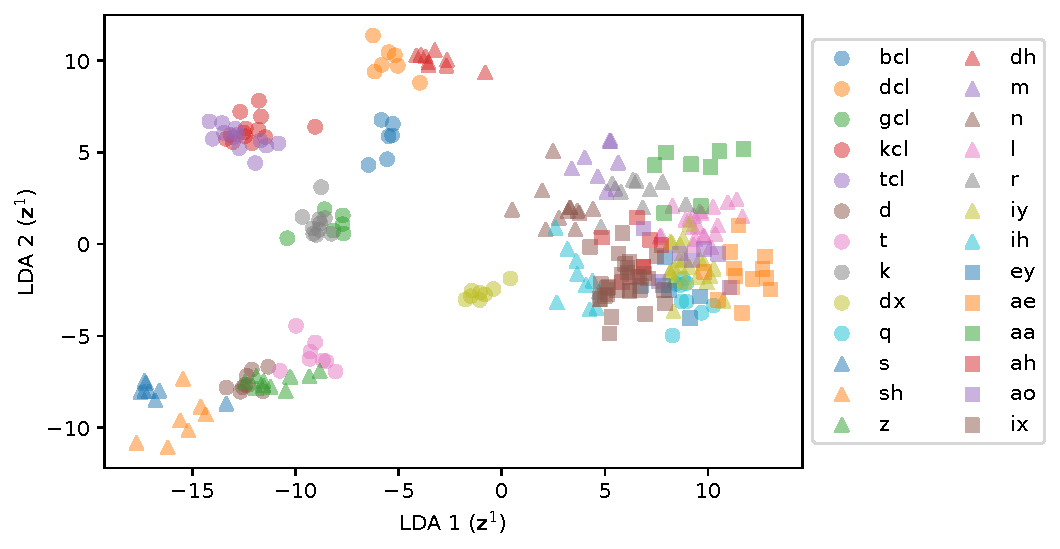
\includegraphics[width=0.555\textwidth]{
        graphics/1xrnjn5y_speaker_phonemes_drw0_latent_0_samples_100_lda_linear_subspace.pdf
    }
    \hfill
    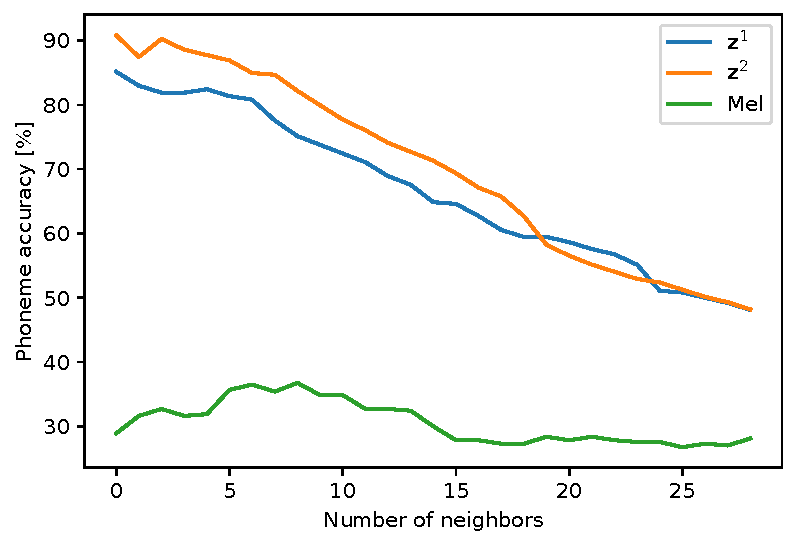
\includegraphics[width=0.425\textwidth]{
        graphics/1xrnjn5y_speaker_phonemes_drw0_samples_100_knn_correct_fraction_model_vs_mel_30_neighbors_lda_subspace_5d.pdf
    }
    \caption{
    (left) Clustering of phonemes in a 2D Linear Discriminant Analysis (LDA) subspace of a CW-VAE latent space ($\vz^{(1)}$).
    (right) Leave-one-out phoneme classification accuracy for a KNN classifier at different $K$ in a 5D LDA subspace of a CW-VAE latent space.
    }
    \label{fig: latent space phoneme and knn}
\end{figure*}


\begin{figure*}[t!]
     \centering
     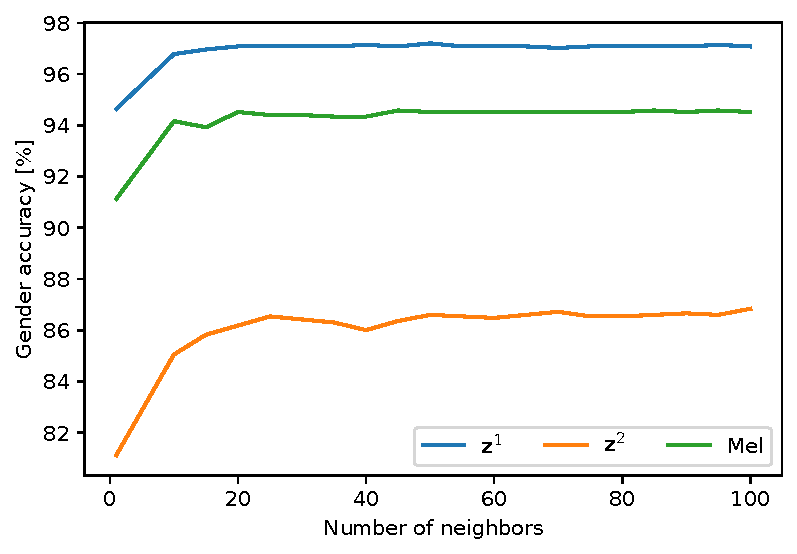
\includegraphics[width=0.477\textwidth]{graphics/1xrnjn5y_speaker_gender_10_samples_knn_correct_fraction_model_vs_mel_100_neighbors_lda_subspace_1d.pdf}
     \hfill
     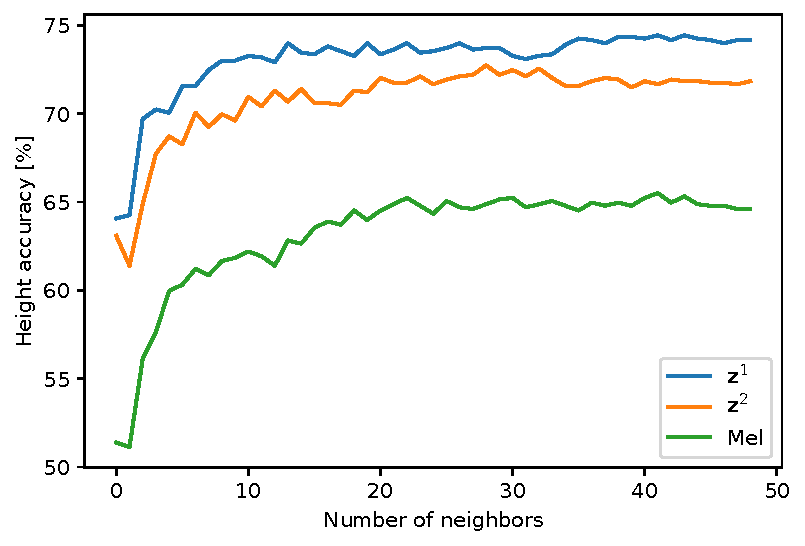
\includegraphics[width=0.483\textwidth]{graphics/1xrnjn5y_speaker_height_m_10_samples_knn_correct_fraction_model_vs_mel_50_neighbors_lda_subspace_2d.pdf}
    \caption{
    Leave-one-out $k$-nearest-neighbor accuracy with different $k$ for
    (a) the speaker's gender and
    (b) the height of male speakers (female speakers yield a similar result).
    }
    \label{fig: knn fraction latent space height and gender}
\end{figure*}


\begin{figure}[t!]
     \centering
     \hfill
     \begin{subfigure}[b]{0.48\textwidth}
         \centering
         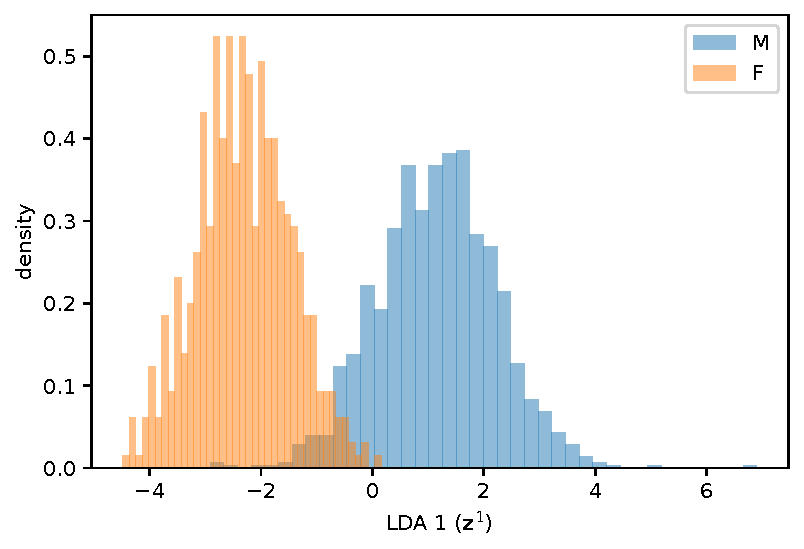
\includegraphics[width=\textwidth]{graphics/1xrnjn5y_speaker_gender_latent_0_1_samples_lda_linear_subspace.pdf}
         \caption{}
         \label{fig: latent space gender}
     \end{subfigure}
     \hfill
     \begin{subfigure}[b]{0.48\textwidth}
         \centering
         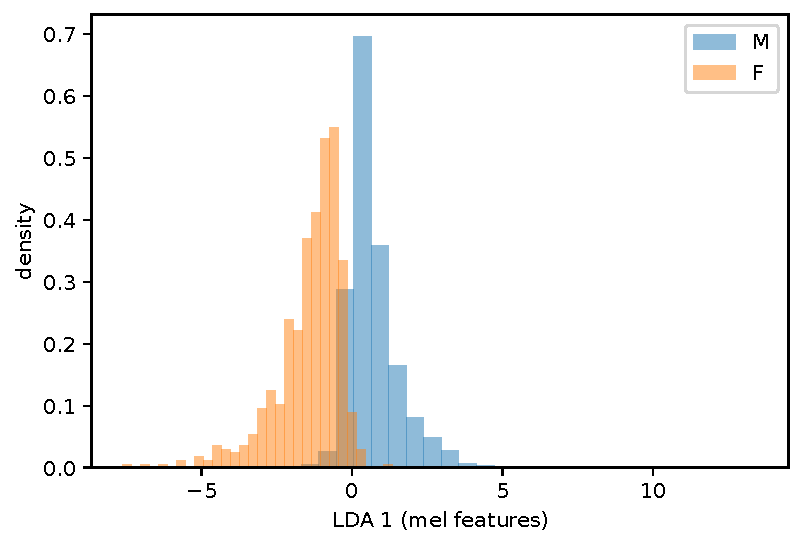
\includegraphics[width=\textwidth]{graphics/1xrnjn5y_speaker_gender_mel_features_lda_linear_subspace.pdf}
         \caption{}
         \label{fig: mel features gender}
     \end{subfigure}
    \caption{Clustering of speaker gender in an one-dimensional linear subspace defined by a linear discriminant analysis of the CW-VAE latent space and of a time-averaged mel spectrogram. The total overlap is slightly smaller in the subspace of the CW-VAE latent space and the separation between the distribution peaks is larger.}
    \label{fig: latent space visualization gender}
\end{figure}


\begin{figure}[t!]
     \centering
     \hfill
     \begin{subfigure}[b]{0.48\textwidth}
         \centering
         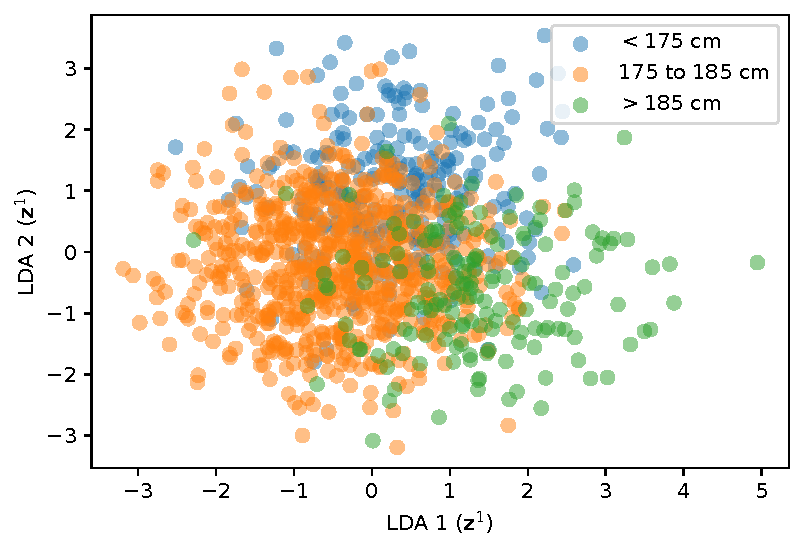
\includegraphics[width=\textwidth]{graphics/1xrnjn5y_speaker_height_m_1_samples_latent_0_lda_linear_subspace.pdf}
         \caption{}
         \label{fig: cwvae latent z1 height}
     \end{subfigure}
     \hfill
     \begin{subfigure}[b]{0.48\textwidth}
         \centering
         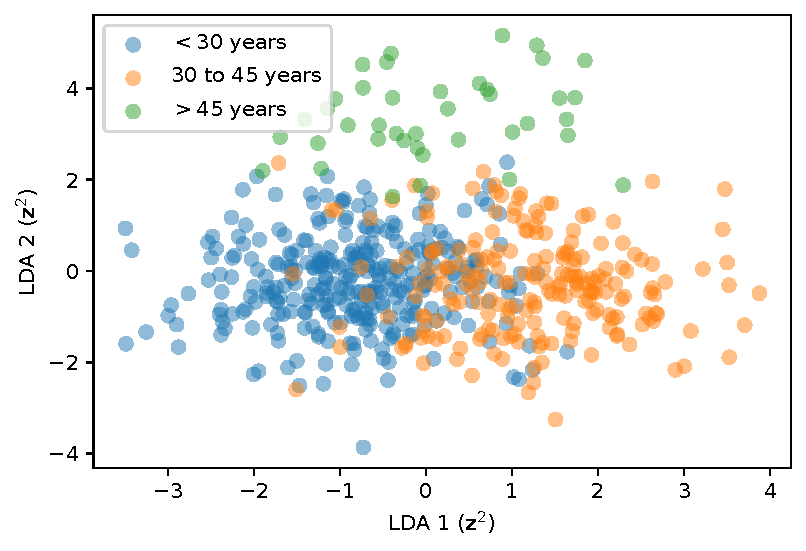
\includegraphics[width=\textwidth]{graphics/1xrnjn5y_speaker_age_f_1_samples_latent_1_lda_linear_subspace.pdf}
         \caption{}
         \label{fig: cwvae latent z0 age}
     \end{subfigure}
    \caption{(a) Clustering of speaker height for male speakers and (b) speaker age for female speakers in an two-dimensional linear subspace defined by a linear discriminant analysis of the CW-VAE latent space.}
    \label{fig: cwvae latent height}
\end{figure}




\section{Distribution of phoneme duration in TIMIT}\label{app: timit phoneme distributions}
In \cref{fig: timit validation set phoneme duration} we plot a boxplots of the duration of each phoneme in the TIMIT dataset. We do this globally as well as for a single speaker to show that phoneme duration can vary between individual speakers. 

A description of the phonemes used for the TIMIT dataset can be found at \url{https://catalog.ldc.upenn.edu/docs/LDC93S1/PHONCODE.TXT}.

\begin{figure}[t!]
    \centering
    \hfill
    \begin{subfigure}[b]{\textwidth}
        \centering
        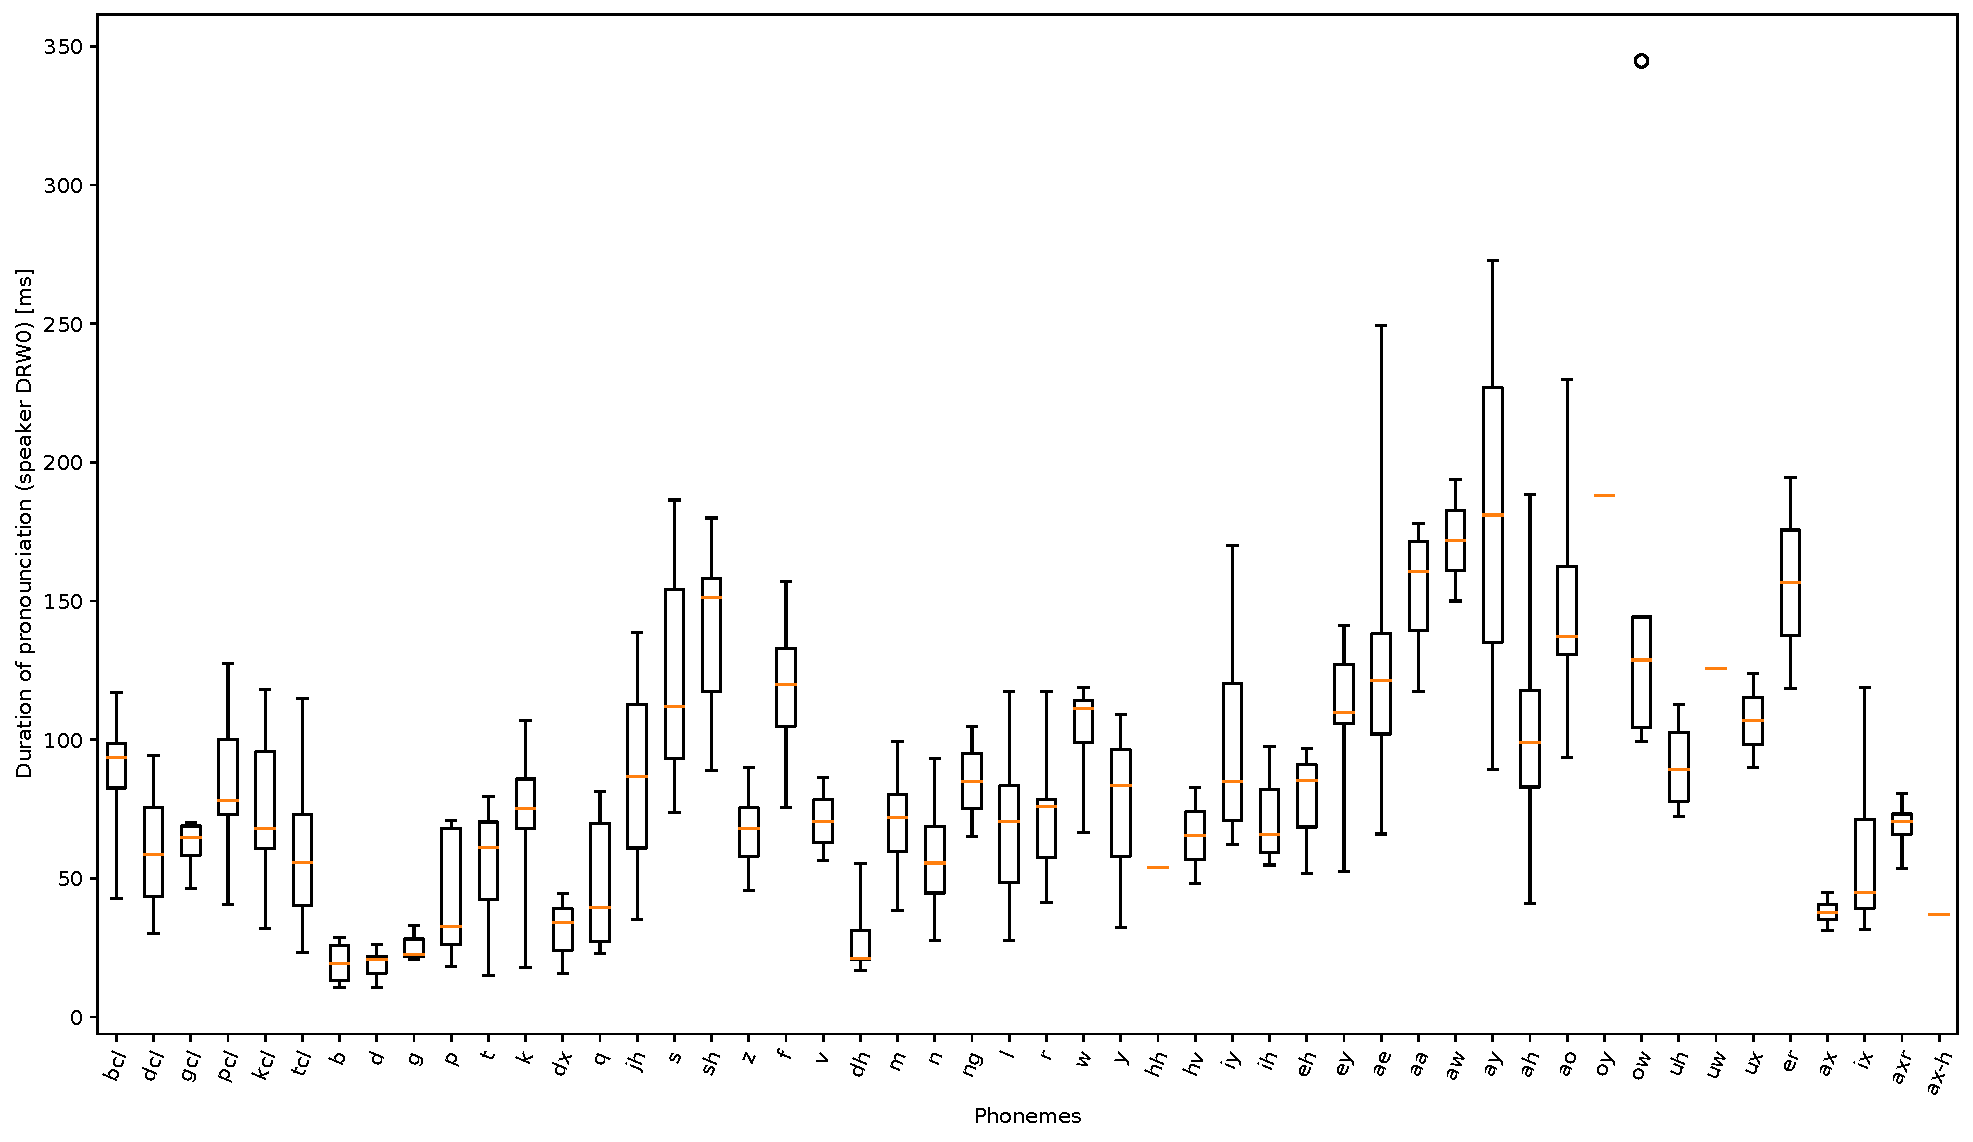
\includegraphics[width=\textwidth]{graphics/timit_validation_set_phoneme_duration_boxplot_speaker_id_drw0.pdf}
        \caption{}
        \label{fig: timit validation set phoneme duration DRW0}
    \end{subfigure}
    \begin{subfigure}[b]{\textwidth}
        \centering
        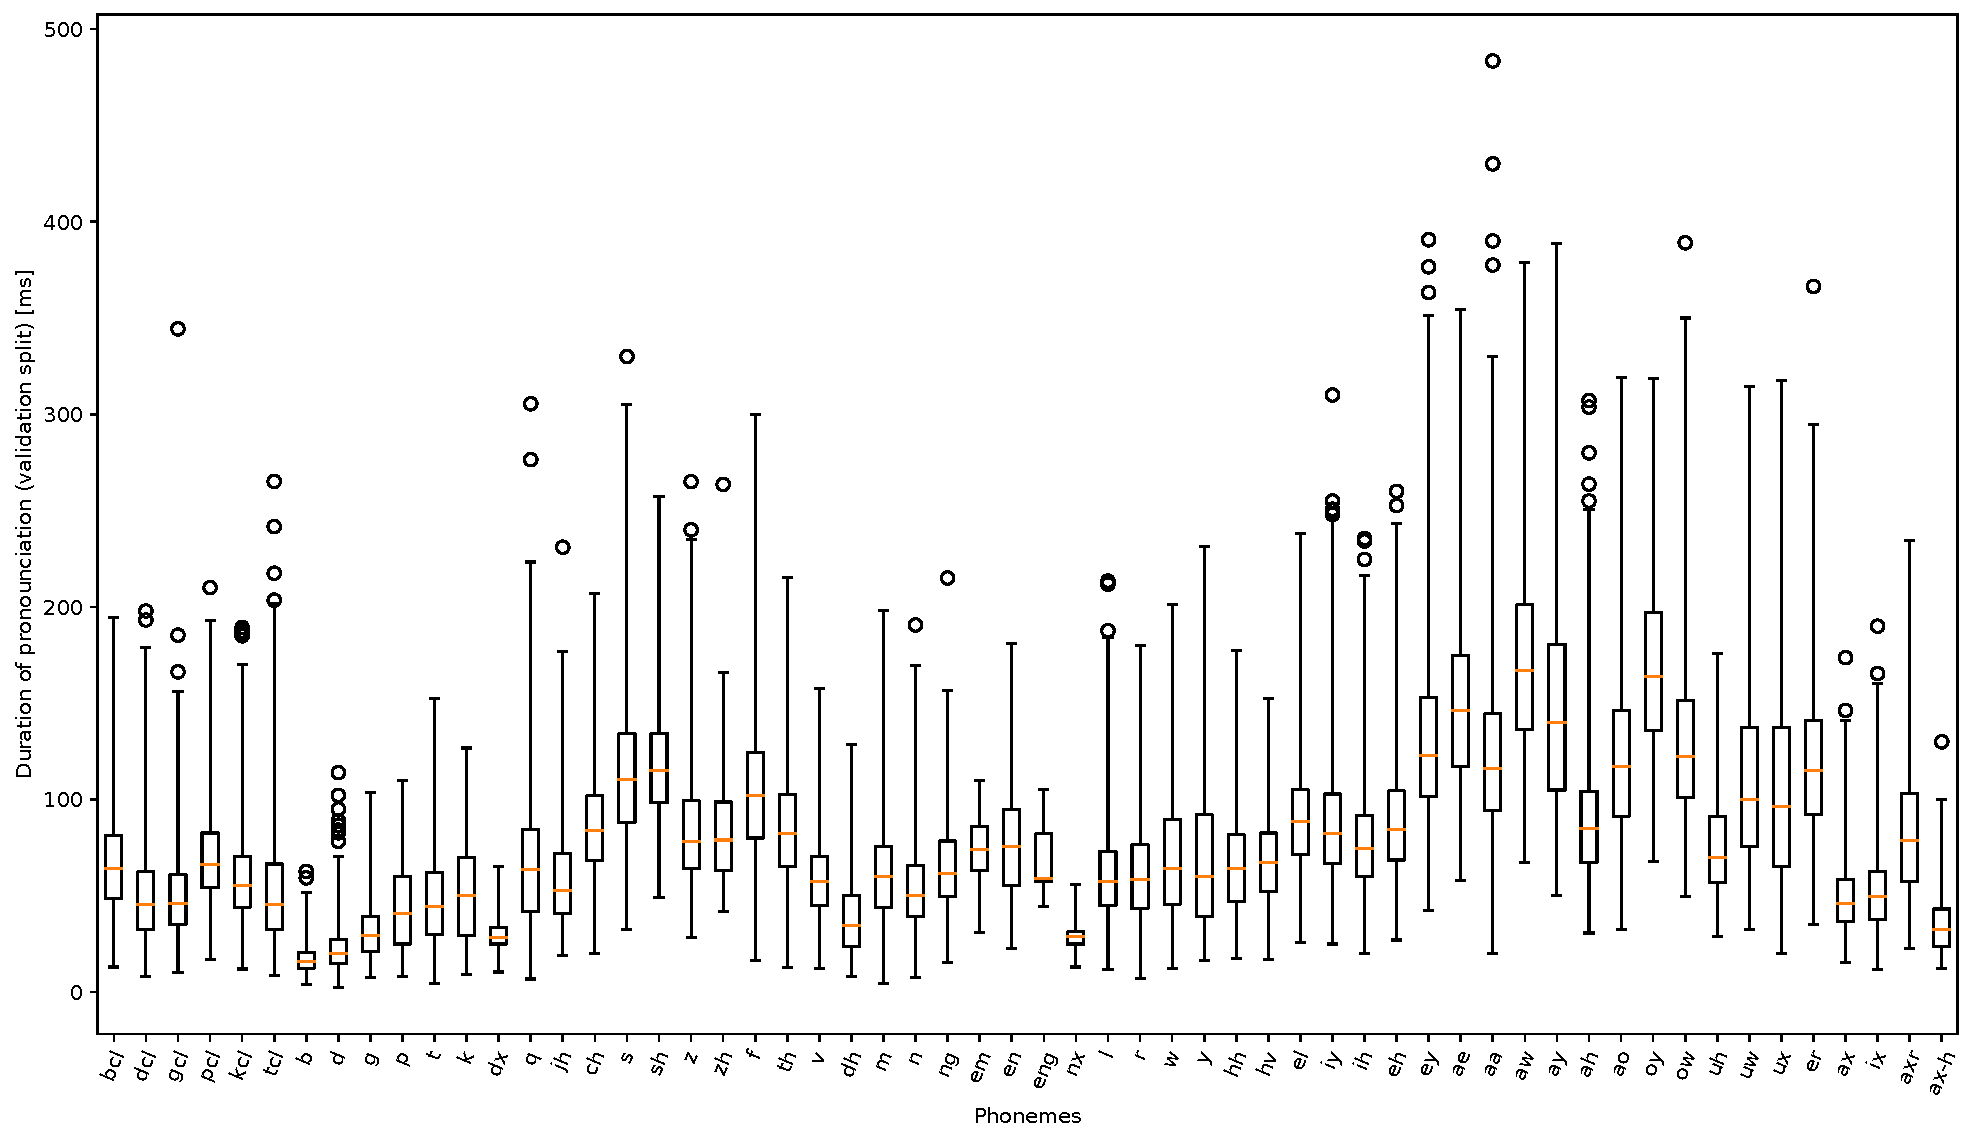
\includegraphics[width=\textwidth]{graphics/timit_validation_set_phoneme_duration_boxplot_speaker_id_none.pdf}
        \caption{}
        \label{fig: timit validation set phoneme duration global}
    \end{subfigure}
    \caption{Boxplots of the duration of the pronunciation of phonemes in TIMIT for a specific speaker DRW0 in (\subref{fig: timit validation set phoneme duration DRW0}) and globally in (\subref{fig: timit validation set phoneme duration global}). Not all phonemes are pronounced by speaker DRW0 over the course of their 10 test set sentences and hence they are missing from the x-axis compared to the global durations.}
    \label{fig: timit validation set phoneme duration}
\end{figure}

\section{Model samples and reconstructions}\label{app: model samples and reconstructions}
We provide samples and reconstructions for some of the models considered here at the following URL: \url{https://doi.org/10.5281/zenodo.5704512}.
The samples are generated from the prior of Clockwork VAE, SRNN and VRNN and from a WaveNet by conditioning on pure zeros. All models are configured as those reported in \cref{tab: likelihoods timit}.
Importantly, the samples are unconditional. Hence they are \emph{not} reconstructions inferred from a given input nor are they conditioned on any auxiliary data like text.

Although sample quality is a somewhat subjective matter, we find the quality of the unconditional Clockwork VAE to be better than those of our VRNN and SRNN. WaveNet is known to produce samples with intelligible speech when conditioned on e.g. text, but unconditional samples from WaveNet lack semantic content such as words as do VRNN, SRNN and Clockwork VAE.

}